\chapter{Specifikacija programske potpore}
		
	\section{Funkcionalni zahtjevi}
			\noindent \textbf{Dionici:}
			\begin{packed_enum}
				\item Pružatelji zdravstvenih usluga (klinike)
				\item Pružatelji prijevoznih usluga (prijevoznici)
				\item Klijenti zdravstvenog turizma (pacijenti)
				\item Korisnici (administratori)
				\begin{packed_enum}
					\item[a)] administratori smještaja
					\item[b)] administratori prijevoza
					\item[c)] korisnički administratori
				\end{packed_enum}
				\item Razvojni tim
			\end{packed_enum}
			
			\noindent \textbf{Aktori i njihovi funkcionalni zahtjevi:}
			\begin{packed_enum}
				\item  \underbar{Neprijavljeni korisnik (inicijator) može:}
				\begin{packed_enum}
					\item se prijaviti na postojeći korisnički račun upisivanjem korisničkog imena i lozinke
				\end{packed_enum}
			
				\item  \underbar{Administrator smještaja (inicijator) može:}
				\begin{packed_enum}
					\item unijeti, modificirati i brisati podatke o smještaju
					\item vidjeti postojeće smještaje, njihove podatke i raspoloživost (uz grafički prikaz)
					\item unijeti i brisati podatke o prijavljenim klinikama
					\item vidjeti postojeće prijavljene klinike
					\item vidjeti postojeće korisnike
					\item registrirati nove korisnike te dodjeljivati uloge i brisati postojeće
				\end{packed_enum}
				
				\item  \underbar{Administrator prijevoznih usluga (inicijator) može:}
				\begin{packed_enum}
					\item unijeti i brisati podatke o prijevoznicima
					\item modificirati podatke raspoloživosti prijevoznika
					\item vidjeti postojeće podatke prijevoznika i njihove raspoloživosti
				\end{packed_enum}
				
				\item  \underbar{Korisnički administrator (inicijator) može:}
				\begin{packed_enum}
					\item unijeti i brisati podatke pacijenata
					\item vidjeti postojeće pacijente i njihove podatke
					\item preuzeti i vidjeti detalje tretmana klinika u kontekstu određenog pacijenta
				\end{packed_enum}
				
					\item  \underbar{Baza podataka (sudionik):}
				\begin{packed_enum}
					\item pohranjuje sve podatke o korisnicima i njihovim ovlastima
					\item pohranjuje sve podatke o smještajima, raspoloživosti i smještajnim kapacitetima
					\item pohranjuje sve podatke o prijevoznicima
					\item pohranjuje sve podatke o pacijentima
					\item pohranjuje sve podatke o dogovorenim terminima boravka pacijenta i prijevoza tijekom boravka
				\end{packed_enum}
			\end{packed_enum}
			\eject 
			
			
			
			\subsection{Obrasci uporabe}
				
				\subsubsection{Opis obrazaca uporabe}
					\textit{Funkcionalne zahtjeve razraditi u obliku obrazaca uporabe. Svaki obrazac je potrebno razraditi prema donjem predlošku. Ukoliko u nekom koraku može doći do odstupanja, potrebno je to odstupanje opisati i po mogućnosti ponuditi rješenje kojim bi se tijek obrasca vratio na osnovni tijek.}\\
					
					% Prijava u sustav
					\noindent \underbar{\textbf{UC1 - Prijava u sustav}}
					\begin{packed_item}
						\item \textbf{Glavni sudionik:} Neprijavljeni korisnik
						\item  \textbf{Cilj:} Dobiti pristup sustavu
						\item  \textbf{Sudionici:} Baza podataka
						\item  \textbf{Preduvjeti:}
						\item[] \begin{packed_enum}
							\item Postojanje korisničkog računa u bazi
						\end{packed_enum}
						
						\item  \textbf{Opis osnovnog tijeka:}
						\item[] \begin{packed_enum}
							\item Unos korisničkog imena i lozinke
							\item Sustav potvrđuje ispravnost unesenih podataka
							\item Sustav omogućava pristup funkcijama definirane ulogom korisničkog računa
						\end{packed_enum}
						
						\item  \textbf{Opis mogućih odstupanja:}
						\item[] \begin{packed_item}
							\item[2.a] Neispravni podaci
							\item[] \begin{packed_enum}
								\item Aplikacija obavještava korisnika o neuspjeloj prijavi prikazivanjem poruke: "Incorrect username or password"
									\end{packed_enum}
						\end{packed_item}
					\end{packed_item}
					
					
					% ---- Korisnici
					% Dodavanje novog korisnika
					\noindent \underbar{\textbf{UC2 - Dodavanje novog korisnika}}
					\begin{packed_item}
						\item \textbf{Glavni sudionik:} Smještajni korisnik
						\item  \textbf{Cilj:} Kreiranje i dodavanje novog korisnika
						\item  \textbf{Sudionici:} Baza podataka
						\item  \textbf{Preduvjeti:}
						\item[] \begin{packed_enum}
							\item Korisnik je prijavljen na račun sa ulogom smještajnog administratora
						\end{packed_enum}
						
						\item  \textbf{Opis osnovnog tijeka:}
						\item[] \begin{packed_enum}
							\item Korisnik odabere opciju "Add new user"
							\item Aplikacija ponuđuje formu za popunjavanje informacija o novom korisniku
							\item Korisnik unosi sve tražene podatke: osobne podatke (\textit{PIN, name, surname, phone} i \textit{e-mail}) i korisničko-specifične podatke (\textit{username, password i role})
							\item Sustav u bazi stvara novog korisnika sa predanim podacima
						\end{packed_enum}
						
						\item  \textbf{Opis mogućih odstupanja:}
						\item[] \begin{packed_item}
							\item[3.a] Unos postojećeg \textit{username}-a
							\item[] \begin{packed_enum}
								\item Aplikacija obavještava korisnika o zauzetosti ponuđenog username-a porukom „Username already in use“
									\end{packed_enum}
							\item[3.b] Krivi format danog osobnog identifikacijskog broja (\textit{PIN}), broja mobitela (\textit{phone number}) ili adrese elektroničke pošte (\textit{e-mail})
							\item[] \begin{packed_enum}
								\item Aplikacija obavještava korisnika o neispravnom formatu i sustav ne ažurira pripadajuće podatke u bazi podataka
									\end{packed_enum}
						\end{packed_item}
					\end{packed_item}
					
					% Pregled korisnika
					\noindent \underbar{\textbf{UC3 - Pregled korisnika}}
					\begin{packed_item}
						\item \textbf{Glavni sudionik:} Smještajni korisnik
						\item  \textbf{Cilj:} Pregled postojećih korisnika
						\item  \textbf{Sudionici:} Baza podataka
						\item  \textbf{Preduvjeti:}
						\item[] \begin{packed_enum}
							\item Korisnik je prijavljen na račun sa ulogom smještajnog administratora
						\end{packed_enum}
						
						\item  \textbf{Opis osnovnog tijeka:}
						\item[] \begin{packed_enum}
							\item Korisnik odabere opciju „View existing users“
							\item Aplikacija prikazuje podatke postojećih korisnika
						\end{packed_enum}
					\end{packed_item}
					
					% Modificiranje podataka korisnika
					\noindent \underbar{\textbf{UC4 - Modificiranje podataka korisnika}}
					\begin{packed_item}
						\item \textbf{Glavni sudionik:} Smještajni korisnik
						\item  \textbf{Cilj:} Modificiranje podataka ciljanog korisnika
						\item  \textbf{Sudionici:} Baza podataka
						\item  \textbf{Preduvjeti:}
						\item[] \begin{packed_enum}
							\item Korisnik je prijavljen na račun sa ulogom smještajnog administratora
							\item Baza sadrži podatke o ciljanom korisniku
						\end{packed_enum}
						
						\item  \textbf{Opis osnovnog tijeka:}
						\item[] \begin{packed_enum}
							\item Korisnik odabere opciju „Modify user info“ pored podataka ciljanog korisnika
							\item Aplikacija ponuđuje formu za popunjavanje i izmjenjivanje informacija o korisniku
							\item Korisnik može izmijeniti osobne podatke (\textit{phone number} i \textit{e-mail}) i korisničko-specifične podatke (\textit{password} i \textit{role})
							\item Sustav u bazi ažurira podatke ciljanog korisnika
						\end{packed_enum}
					\end{packed_item}
				
					% Brisanje postojećeg korisnika
					\noindent \underbar{\textbf{UC5 - Brisanje postojeće korisnika}}
					\begin{packed_item}
						\item \textbf{Glavni sudionik:} Smještajni korisnik
						\item  \textbf{Cilj:} Brisanje ciljanog korisnika
						\item  \textbf{Sudionici:} Baza podataka
						\item  \textbf{Preduvjeti:}
						\item[] \begin{packed_enum}
							\item Korisnik je prijavljen na račun sa ulogom smještajnog administratora
							\item Baza sadrži podatke o ciljanom korisniku
						\end{packed_enum}
						
						\item  \textbf{Opis osnovnog tijeka:}
						\item[] \begin{packed_enum}
							\item Korisnik odabere opciju „Delete“ pokraj podataka ciljanog korisnika
							\item Korisnik potvrđuje odabir nakon upita aplikacije
							\item Sustav briše podatke odabranog korisnika iz baze
						\end{packed_enum}
						
						\item  \textbf{Opis mogućih odstupanja:}
						\item[] \begin{packed_item}
							\item[2.a] Korisnik odustane od brisanja tijekom procesa brisanja
							\item[] \begin{packed_enum}
								\item Aplikacija obavještava korisnika o prekidu brisanja
									\end{packed_enum}
						\end{packed_item}
					\end{packed_item}
					
					
					% ---- Smještaj
					% Dodavanje novog smještaja
					\noindent \underbar{\textbf{UC6 - Dodavanje novog smještaja}}
					\begin{packed_item}
						\item \textbf{Glavni sudionik:} Smještajni korisnik
						\item  \textbf{Cilj:} Kreiranje i dodavanje novog smještaja
						\item  \textbf{Sudionici:} Baza podataka
						\item  \textbf{Preduvjeti:}
						\item[] \begin{packed_enum}
							\item Korisnik je prijavljen na račun sa ulogom smještajnog administratora
						\end{packed_enum}
						
						\item  \textbf{Opis osnovnog tijeka:}
						\item[] \begin{packed_enum}
							\item Korisnik odabere opciju „Add new accomodation“
							\item Sustav ponuđuje formu za popunjavanje informacija o novom smještaju
							\item Korisnik unosi tražene podatke: osnovne podatke (\textit{address, latitude, longitude, accomodation type} i \textit{equipment category}) i da li je smještaj raspoloživ (\textit{active})
							\item Sustav u bazi stvara novi smještaj sa predanim podacima
						\end{packed_enum}
						
						\item  \textbf{Opis mogućih odstupanja:}
						\item[] \begin{packed_item}
							\item[3.a] Unos postojeće adrese (\textit{address}) ili geografske pozicije (\textit{latitude} i \textit{longitude})
							\item[] \begin{packed_enum}
								\item Aplikacija obavještava korisnika o već postojećim unesenim podatcima u bazi
							\end{packed_enum}
						\end{packed_item}
					\end{packed_item}
					
					% Pregled smještaja
					\noindent \underbar{\textbf{UC7 - Pregled smještaja}}
					\begin{packed_item}
						\item \textbf{Glavni sudionik:} Smještajni korisnik
						\item  \textbf{Cilj:} Pregled unesenih smještaja
						\item  \textbf{Sudionici:} Baza podataka
						\item  \textbf{Preduvjeti:}
						\item[] \begin{packed_enum}
							\item Korisnik je prijavljen na račun sa ulogom smještajnog administratora
						\end{packed_enum}
						
						\item  \textbf{Opis osnovnog tijeka:}
						\item[] \begin{packed_enum}
							\item Korisnik odabere opciju „View accomodations“
							\item Aplikacija prikazuje podatke unesenih smještaja, uključujući prikaz geografske lokacije smještaja na karti
						\end{packed_enum}
					\end{packed_item}
					
					% Postavljanje raspoloživosti smještaja
					\noindent \underbar{\textbf{UC8 - Postavljanje raspoloživosti smještaja}}
					\begin{packed_item}
						\item \textbf{Glavni sudionik:} Smještajni korisnik
						\item  \textbf{Cilj:} Postavljanje željene raspoloživosti smještaja
						\item  \textbf{Sudionici:} Baza podataka
						\item  \textbf{Preduvjeti:}
						\item[] \begin{packed_enum}
							\item Korisnik je prijavljen na račun sa ulogom smještajnog administratora
						\end{packed_enum}
						
						\item  \textbf{Opis osnovnog tijeka:}
						\item[] \begin{packed_enum}
							\item Korisnik postavlja raspoloživost smještaja pomoću potvrdnog okvira
							\item Sustav u bazi ažurira raspoloživost smještaja
						\end{packed_enum}
					\end{packed_item}
					
					% Brisanje postojećeg korisnika
					\noindent \underbar{\textbf{UC9 - Brisanje postojećeg smještaja}}
					\begin{packed_item}
						\item \textbf{Glavni sudionik:} Smještajni korisnik
						\item  \textbf{Cilj:} Brisanje ciljanog smještaja
						\item  \textbf{Sudionici:} Baza podataka
						\item  \textbf{Preduvjeti:}
						\item[] \begin{packed_enum}
							\item Korisnik je prijavljen na račun sa ulogom smještajnog administratora
							\item Baza sadrži podatke o ciljanom smještaju
						\end{packed_enum}
						
						\item  \textbf{Opis osnovnog tijeka:}
						\item[] \begin{packed_enum}
							\item Korisnik odabere opciju „Remove accomodation“ pokraj podataka ciljanog smještaja
							\item Korisnik potvrđuje odabir nakon upita aplikacije
							\item Sustav briše podatke odabranog smještaja iz baze
						\end{packed_enum}
						
						\item  \textbf{Opis mogućih odstupanja:}
						\item[] \begin{packed_item}
							\item[2.a] Korisnik odustane od brisanja tijekom procesa brisanja
							\item[] \begin{packed_enum}
								\item Aplikacija obavještava korisnika o prekidu brisanja
							\end{packed_enum}
						\end{packed_item}
					\end{packed_item}
					
					
					% ---- Prijevoznici
					% Dodavanje novog prijevoznika
					\noindent \underbar{\textbf{UC10 - Dodavanje novog smještaja}}
					\begin{packed_item}
						\item \textbf{Glavni sudionik:} Administrator prijevoznih usluga
						\item  \textbf{Cilj:} Kreiranje i dodavanje novog prijevoznika
						\item  \textbf{Sudionici:} Baza podataka
						\item  \textbf{Preduvjeti:}
						\item[] \begin{packed_enum}
							\item Korisnik je prijavljen na račun sa ulogom administratora prijevoznih usluga
						\end{packed_enum}
						
						\item  \textbf{Opis osnovnog tijeka:}
						\item[] \begin{packed_enum}
							\item Korisnik odabere opciju „Add new transporter“
							\item Aplikacija ponuđuje formu za popunjavanje informacija o novom prijevozniku
							\item Korisnik unosi tražene osobne i kontaktne podatke prijevoznika (\textit{phone number, organization name, address} i \textit{active})
							\item Sustav u bazu sprema podatke o prijevozniku
						\end{packed_enum}
						
						\item  \textbf{Opis mogućih odstupanja:}
						\item[] \begin{packed_item}
							\item[3.a] Krivi format danog broja mobitela (\textit{phone number})
							\item[] \begin{packed_enum}
								\item Aplikacija obavještava korisnika o neispravnom formatu i ne ažurira pripadajuće podatke u bazi podataka
							\end{packed_enum}
						\end{packed_item}
					\end{packed_item}
					
					% Pregled prijevoznika
					\noindent \underbar{\textbf{UC11 - Pregled smještaja}}
					\begin{packed_item}
						\item \textbf{Glavni sudionik:} Administrator prijevoznih usluga
						\item  \textbf{Cilj:} Pregled unesenih prijevoznika
						\item  \textbf{Sudionici:} Baza podataka
						\item  \textbf{Preduvjeti:}
						\item[] \begin{packed_enum}
							\item Korisnik je prijavljen na račun sa ulogom administratora prijevoznih usluga
						\end{packed_enum}
						
						\item  \textbf{Opis osnovnog tijeka:}
						\item[] \begin{packed_enum}
							\item Korisnik odabere opciju „View transporters“
							\item Aplikacija prikazuje podatke unesenih prijevoznika
						\end{packed_enum}
					\end{packed_item}
					
					% Brisanje postojećeg korisnika
					\noindent \underbar{\textbf{UC12 - Brisanje postojećeg smještaja}}
					\begin{packed_item}
						\item \textbf{Glavni sudionik:} Administrator prijevoznih usluga
						\item  \textbf{Cilj:} Brisanje ciljanog prijevoznika
						\item  \textbf{Sudionici:} Baza podataka
						\item  \textbf{Preduvjeti:}
						\item[] \begin{packed_enum}
							\item Korisnik je prijavljen na račun sa ulogom administratora prijevoznih usluga
							\item Baza sadrži podatke ciljanog prijevoznika
						\end{packed_enum}
						
						\item  \textbf{Opis osnovnog tijeka:}
						\item[] \begin{packed_enum}
							\item Korisnik odabere opciju „Delete“ pokraj podataka ciljanog prijevoznika
							\item Korisnik potvrđuje odabir nakon upita aplikacije
							\item Sustav briše podatke odabranog smještaja iz baze
						\end{packed_enum}
					
						\item  \textbf{Opis mogućih odstupanja:}
						\item[] \begin{packed_item}
							\item[2.a] Korisnik odustane od brisanja tijekom procesa brisanja
							\item[] \begin{packed_enum}
								\item Aplikacija obavještava korisnika o prekidu brisanja
							\end{packed_enum}
						\end{packed_item}
					\end{packed_item}
					
					% Dodavanje vozila prijevoznika
					\noindent \underbar{\textbf{UC13 - Dodavanje vozila prijevoznika}}
					\begin{packed_item}
						\item \textbf{Glavni sudionik:} Administrator prijevoznih usluga
						\item  \textbf{Cilj:} Kreiranje i dodavanje novog vozila prijevoznika
						\item  \textbf{Sudionici:} Baza podataka
						\item  \textbf{Preduvjeti:}
						\item[] \begin{packed_enum}
							\item Korisnik je prijavljen na račun sa ulogom administratora prijevoznih usluga
						\end{packed_enum}
						
						\item  \textbf{Opis osnovnog tijeka:}
						\item[] \begin{packed_enum}
							\item Korisnik odabere opciju „Add new vehicle“ pod podatcima ciljanog prijevoznika
							\item Aplikacija ponuđuje formu za popunjavanje informacija o novom vozilu
							\item Korisnik unosi tražene podatke o vozilu (\textit{type of vehicle, capacity} i \textit{active})
							\item Sustav u bazi stvara novo vozilo i pridjeljuje ga ciljanom prijevozniku
						\end{packed_enum}
					\end{packed_item}
						
					% Pregled vozila prijevoznika
					\noindent \underbar{\textbf{UC14 - Pregled vozila prijevoznika}}
					\begin{packed_item}
						\item \textbf{Glavni sudionik:} Administrator prijevoznih usluga
						\item  \textbf{Cilj:} Pregled unesenih vozila određenog prijevoznika
						\item  \textbf{Sudionici:} Baza podataka
						\item  \textbf{Preduvjeti:}
						\item[] \begin{packed_enum}
							\item Korisnik je prijavljen na račun sa ulogom administratora prijevoznih usluga
						\end{packed_enum}
						
						\item  \textbf{Opis osnovnog tijeka:}
						\item[] \begin{packed_enum}
							\item Korisnik odabere opciju „View assigned vehicles“
							\item Aplikacija prikazuje podatke unesenih vozila ciljanog prijevoznika
						\end{packed_enum}
					\end{packed_item}
					
					% Postavljanje raspoloživosti vozila prijevoznika
					\noindent \underbar{\textbf{UC15 - Postavljanje raspoloživosti vozila prijevoznika}}
					\begin{packed_item}
						\item \textbf{Glavni sudionik:} Administrator prijevoznih usluga
						\item  \textbf{Cilj:} Postavljanje raspoloživosti ciljanog vozila prijevoznik
						\item  \textbf{Sudionici:} Baza podataka
						\item  \textbf{Preduvjeti:}
						\item[] \begin{packed_enum}
							\item Korisnik je prijavljen na račun sa ulogom administratora prijevoznih usluga
						\end{packed_enum}
						
						\item  \textbf{Opis osnovnog tijeka:}
						\item[] \begin{packed_enum}
							\item Korisnik postavlja raspoloživost ciljanog vozila pomoću potvrdnog okvira
							\item Sustav u bazi ažurira raspoloživost ciljanog vozila
						\end{packed_enum}
					\end{packed_item}
					
					% Brisanje vozila prijevoznika
					\noindent \underbar{\textbf{UC16 - Brisanje vozila prijevoznika}}
					\begin{packed_item}
						\item \textbf{Glavni sudionik:} Administrator prijevoznih usluga
						\item  \textbf{Cilj:} Brisanje ciljanog vozila prijevoznika
						\item  \textbf{Sudionici:} Baza podataka
						\item  \textbf{Preduvjeti:}
						\item[] \begin{packed_enum}
							\item Korisnik je prijavljen na račun sa ulogom administratora prijevoznih usluga
							\item Baza sadrži podatke ciljanog vozila ciljanog prijevoznik
						\end{packed_enum}
						
						\item  \textbf{Opis osnovnog tijeka:}
						\item[] \begin{packed_enum}
							\item Korisnik odabere opciju „Remove vehicle“ pod podatcima ciljanog prijevoznika
							\item Korisnik potvrđuje odabir nakon upita aplikacije
							\item Sustav briše podatke odabranog vozila prijevoznika iz baze
						\end{packed_enum}
					
						\item  \textbf{Opis mogućih odstupanja:}
						\item[] \begin{packed_item}
							\item[2.a] Korisnik odustane od brisanja tijekom procesa brisanja
							\item[] \begin{packed_enum}
								\item Aplikacija obavještava korisnika o prekidu brisanja
							\end{packed_enum}
						\end{packed_item}
					\end{packed_item}
					
					% ---- Pacijenti
					% Dodavanje pacijenta
					\noindent \underbar{\textbf{UC17 - Dodavanje pacijenta}}
					\begin{packed_item}
						\item \textbf{Glavni sudionik:} Korisnički administrator
						\item  \textbf{Cilj:} Kreiranje i dodavanje novog pacijenta
						\item  \textbf{Sudionici:} Baza podataka
						\item  \textbf{Preduvjeti:}
						\item[] \begin{packed_enum}
							\item Korisnik je prijavljen na račun sa ulogom korisničkog administratora
						\end{packed_enum}
						
						\item  \textbf{Opis osnovnog tijeka:}
						\item[] \begin{packed_enum}
							\item Korisnik odabere opciju „Add new patient“
							\item Aplikacija ponuđuje formu za popunjavanje informacija o novom pacijentu
							\item Korisnik unosi tražene podatke: osobne i kontaktne podatke (\textit{PIN, name, surname, phone, e-mail} i \textit{residence address}) te podatke o tretmanu (\textit{clinic} i \textit{treatment}) i preferenciji smještaja (\textit{accomodation preferences})
							\item Sustav u bazi stvara novog pacijenta sa predanim podacima
						\end{packed_enum}
						
						\item  \textbf{Opis mogućih odstupanja:}
						\item[] \begin{packed_item}
							\item[3.a] Krivi format danog osobnog identifikacijskog broja (\textit{PIN}), broja mobitela (\textit{phone number}) ili adrese elektroničke pošte (\textit{e-mail})
							\item[] \begin{packed_enum}
								\item Aplikacija obavještava korisnika o neispravnom formatu i ne ažurira pripadajuće podatke u bazi podataka
							\end{packed_enum}
						\end{packed_item}
					\end{packed_item}
					
					% Pregled pacijenata
					\noindent \underbar{\textbf{UC18 - Pregled pacijenataa}}
					\begin{packed_item}
						\item \textbf{Glavni sudionik:} Korisnički administrator
						\item  \textbf{Cilj:} Pregled postojećih pacijenata
						\item  \textbf{Sudionici:} Baza podataka
						\item  \textbf{Preduvjeti:}
						\item[] \begin{packed_enum}
							\item Korisnik je prijavljen na račun sa ulogom korisničkog administratora
						\end{packed_enum}
						
						\item  \textbf{Opis osnovnog tijeka:}
						\item[] \begin{packed_enum}
							\item Korisnik odabere opciju „View patients“
							\item Aplikacija prikazuje podatke postojećih pacijenata, uključujući da li im je pridijeljen smještaj i prijevoz, te podacima o smještaju i prijevozu u slučaju da jesu pridijeljeni
						\end{packed_enum}
					\end{packed_item}
					
					% Dohvaćanje informacija o tretmanu
					\noindent \underbar{\textbf{UC19 - Dohvaćanje informacija o tretmanu}}
					\begin{packed_item}
						\item \textbf{Glavni sudionik:} Sustav
						\item  \textbf{Cilj:} Dohvaćanje informacija o tretmanu pacijenta pri registraciji/dodavanju pacijenta
						\item  \textbf{Sudionici:} Baza podataka, baza podataka pacijentove klinike
						\item  \textbf{Preduvjeti:}
						\item[] \begin{packed_enum}
							\item Baza sadrži sve potrebne podatke o pacijentu
							\item Baza podataka klinike sadrži potrebne podatke o tretmanu pacijenta
						\end{packed_enum}
						
						\item  \textbf{Opis osnovnog tijeka:}
						\item[] \begin{packed_enum}
							\item Sustav uspostavlja vezu sa bazom podataka klinike
							\item Sustav dohvaća podatke o tretmanu iz baze podataka klinike
							\item Sustav sprema dohvaćene podatke u bazu podataka sustava
						\end{packed_enum}
						
						\item  \textbf{Opis mogućih odstupanja:}
						\item[] \begin{packed_item}
							\item[1.a] Sustav ne može uspostaviti vezu sa klinikom
							\item[] \begin{packed_enum}
								\item Aplikacija obavještava korisnika o neuspješnom povezivanju
							\end{packed_enum}
						\end{packed_item}
					\end{packed_item}
					
					% Brisanje pacijenta
					\noindent \underbar{\textbf{UC20 - Brisanje pacijenta}}
					\begin{packed_item}
						\item \textbf{Glavni sudionik:} Korisnički administrator
						\item  \textbf{Cilj:} Brisanje ciljanog vozila prijevoznika
						\item  \textbf{Sudionici:} Baza podataka
						\item  \textbf{Preduvjeti:}
						\item[] \begin{packed_enum}
							\item Korisnik je prijavljen na račun sa ulogom korisničkog administratora
							\item Baza sadrži podatke ciljanog pacijenta
						\end{packed_enum}
						
						\item  \textbf{Opis osnovnog tijeka:}
						\item[] \begin{packed_enum}
							\item Korisnik odabere opciju „Delete“ pokraj podataka ciljanog pacijenta
							\item Korisnik potvrđuje odabir nakon upita aplikacije
							\item Sustav briše podatke odabranog pacijenta iz baze
						\end{packed_enum}
						
						\item  \textbf{Opis mogućih odstupanja:}
						\item[] \begin{packed_item}
							\item[2.a] Korisnik odustane od brisanja tijekom procesa
							\item[] \begin{packed_enum}
								\item Aplikacija obavještava korisnika o prekidu brisanja
							\end{packed_enum}
						\end{packed_item}
					\end{packed_item}
					
					% ---- Ostalo
					% Periodičko pridjeljivanje smještaja i prijevoza pacijentima
					\noindent \underbar{\textbf{UC21 - Periodičko pridjeljivanje smještaja i prijevoza pacijentima}}
					\begin{packed_item}
						\item \textbf{Glavni sudionik:} Korisnički administrator
						\item  \textbf{Cilj:} Pridjeljivanje adekvatnog smještaja i prijevoza upisanim pacijentima te obavještavanje pacijenta o uspješnom pridjeljenju
						\item  \textbf{Sudionici:} Baza podataka
						\item  \textbf{Preduvjeti:}
						\item[] \begin{packed_enum}
							\item Baza sadrži potrebne podatke o pacijentima, smještajima i prijevoznicima
							\item Baza sadrži barem jednu instancu svakog potrebnog podatka
						\end{packed_enum}
						
						\item  \textbf{Opis osnovnog tijeka:}
						\item[] \begin{packed_enum}
							\item Sustav provjerava unesene podatke za pacijente bez smještaja
							\item Sustav (ako je moguće) pridjeljuje adekvatni smještaj pacijentu
							\item Sustav (ako je moguće) pridjeljuje adekvatni prijevoz pacijentu pri zaključenju medicinskog plana
						\end{packed_enum}
						
						\item  \textbf{Opis mogućih odstupanja:}
						\item[] \begin{packed_item}
							\item[2.a] Sustav ne može naći adekvatni smještaj i/ili prijevoz pacijentu
							\item[] \begin{packed_enum}
								\item Sustav periodički pokušava ponovno pri unosu novih podataka
							\end{packed_enum}
						\end{packed_item}
					\end{packed_item}
					
					% Obavještavanje klijenata o uspješnom zaključenju plana
					\noindent \underbar{\textbf{UC22 - Obavještavanje klijenata o uspješnom zaključenju plana}}
					\begin{packed_item}
						\item \textbf{Glavni sudionik:} Sustav
						\item  \textbf{Cilj:} Obavještavanje pacijenta, prijevoznika o uspješno zaključenom planu medicinskih usluga
						\item  \textbf{Sudionici:} Baza podataka, pacijent, prijevoznik
						\item  \textbf{Preduvjeti:}
						\item[] \begin{packed_enum}
							\item Baza sadrži potrebne podatke o pacijentima, smještajima i prijevoznicima
							\item Sustav je uspješno zaključio medicinski plan pacijenta pridjeljivanjem smještaja i prijevoza pacijentu
						\end{packed_enum}
						
						\item  \textbf{Opis osnovnog tijeka:}
						\item[] \begin{packed_enum}
							\item Sustav provjerava zaključen plan te primjereno modificira podatke u bazi podataka (raspoloživost smještaja i vozila prijevoznika)
							\item Aplikacija šalje mail pacijentu sa podacima o datumu plana korištenja tretmana te smještaju i prijevozu tijekom plana tretmana
							\item Aplikacija šalje mail prijevozniku o zauzetosti vozila koje će se koristiti za pridijeljeni medicinski plan
						\end{packed_enum}
					\end{packed_item}
				\break
					
				\subsubsection{Dijagrami obrazaca uporabe}

					\begin{figure}[H]
						\centering
						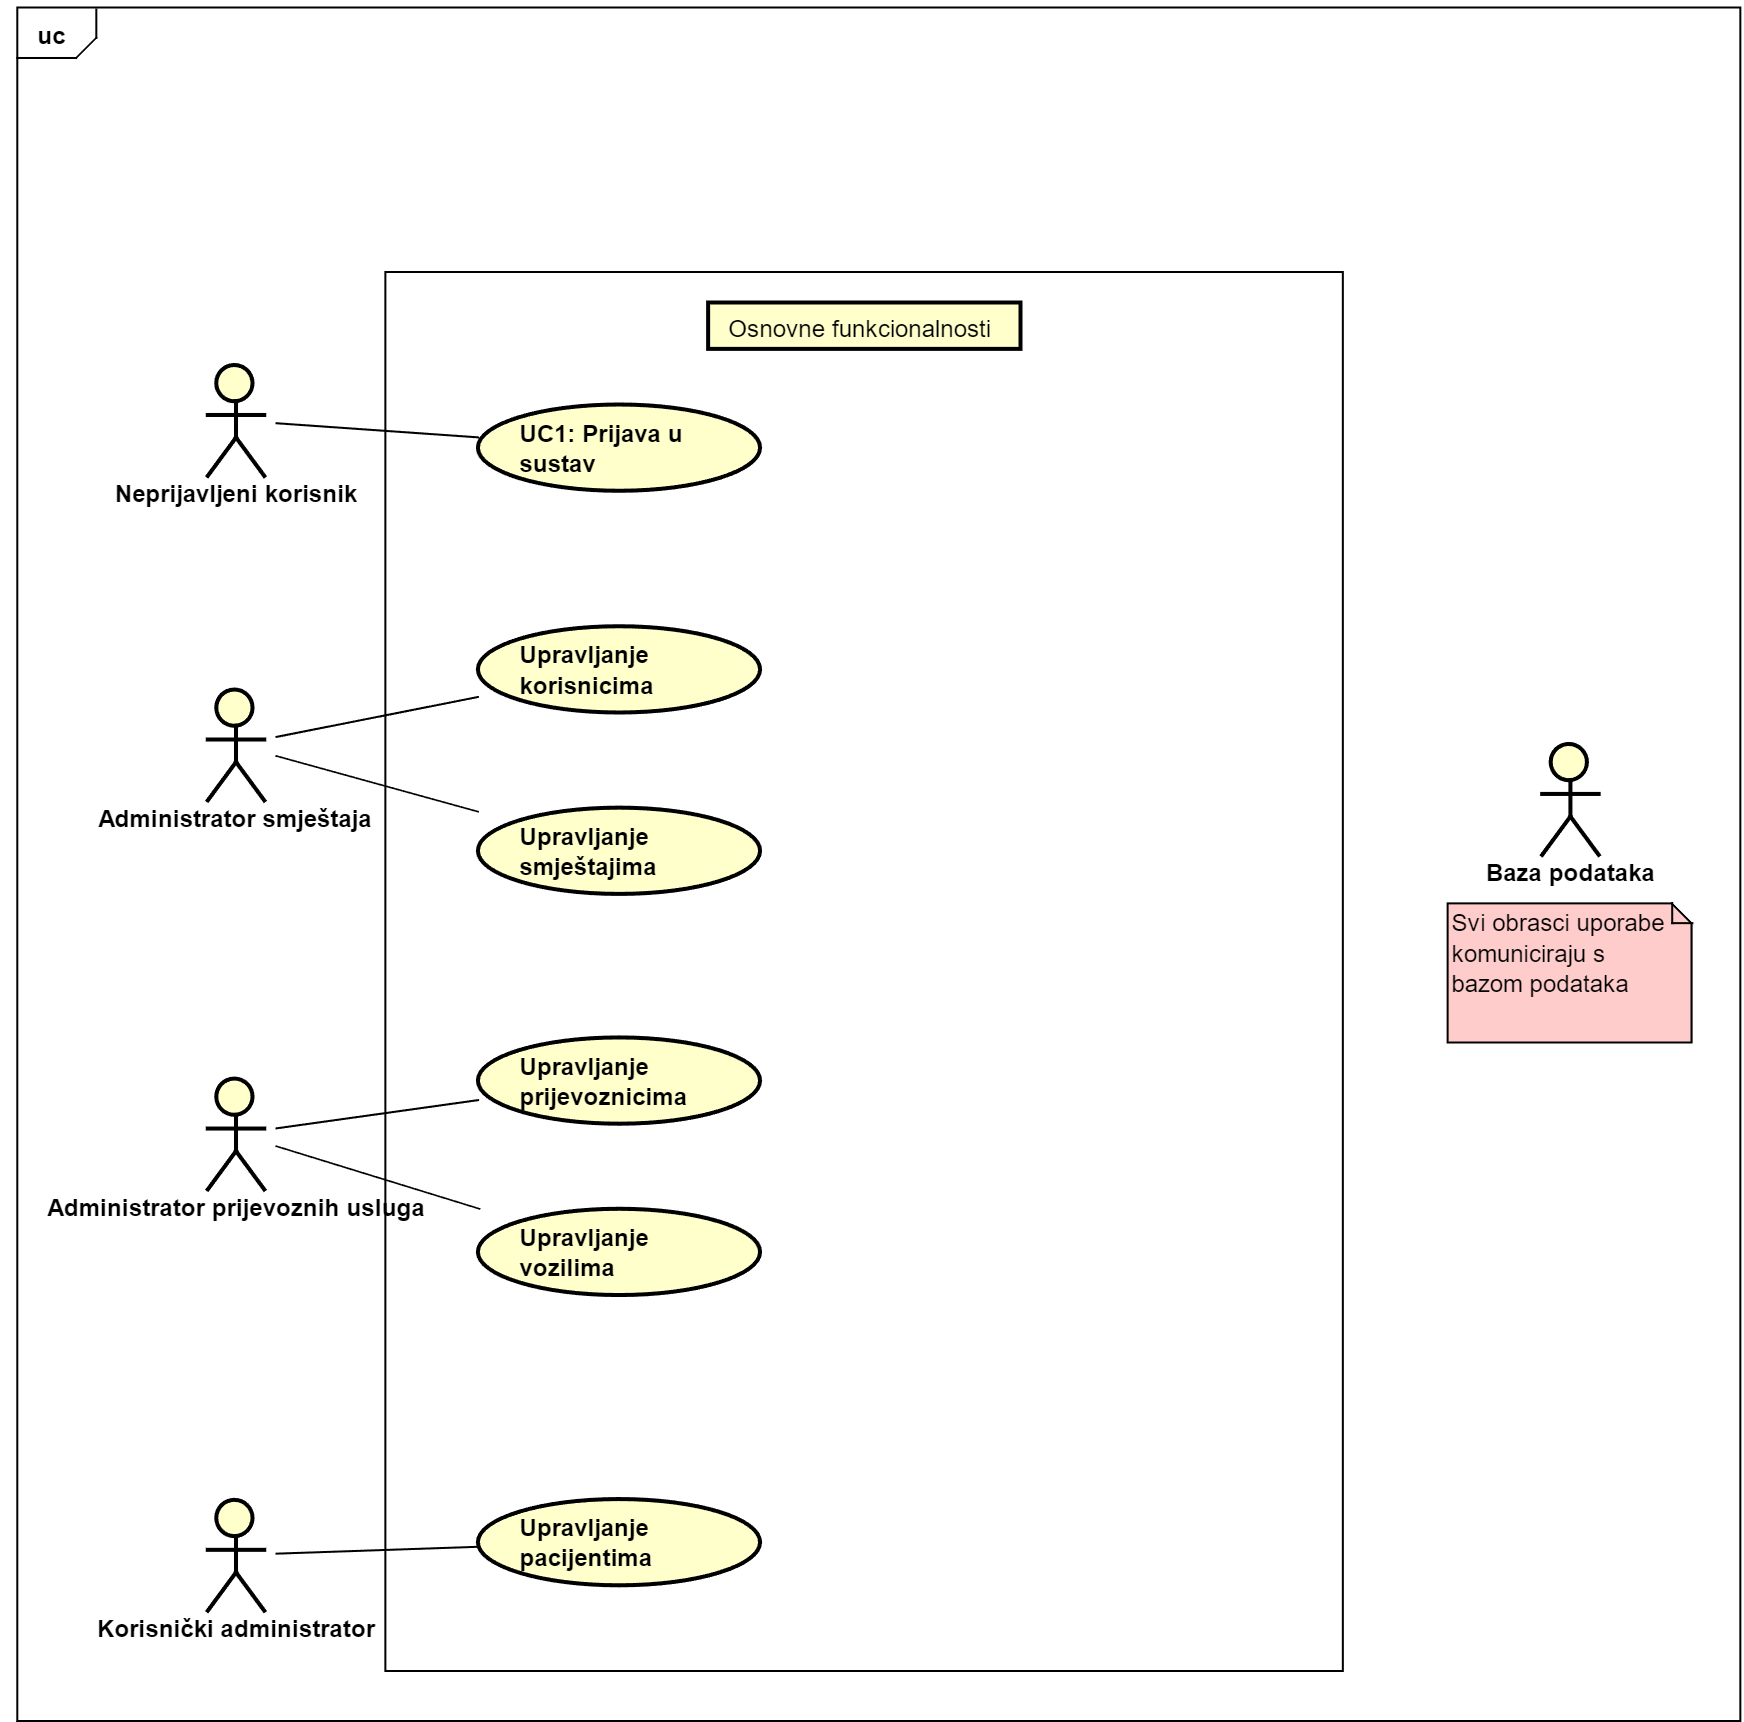
\includegraphics[width=\textwidth]{slike/DOU_OsnovneFunkcionalnosti.png} %veličina slike u odnosu na originalnu datoteku i pozicija slike
						\caption{Dijagram obrasca uporabe, osnovne funkcionalnosti}
						\label{fig:osnovne funkcionalnosti}
					\end{figure}
				\eject		
				
					\begin{figure}[H]
					\centering
					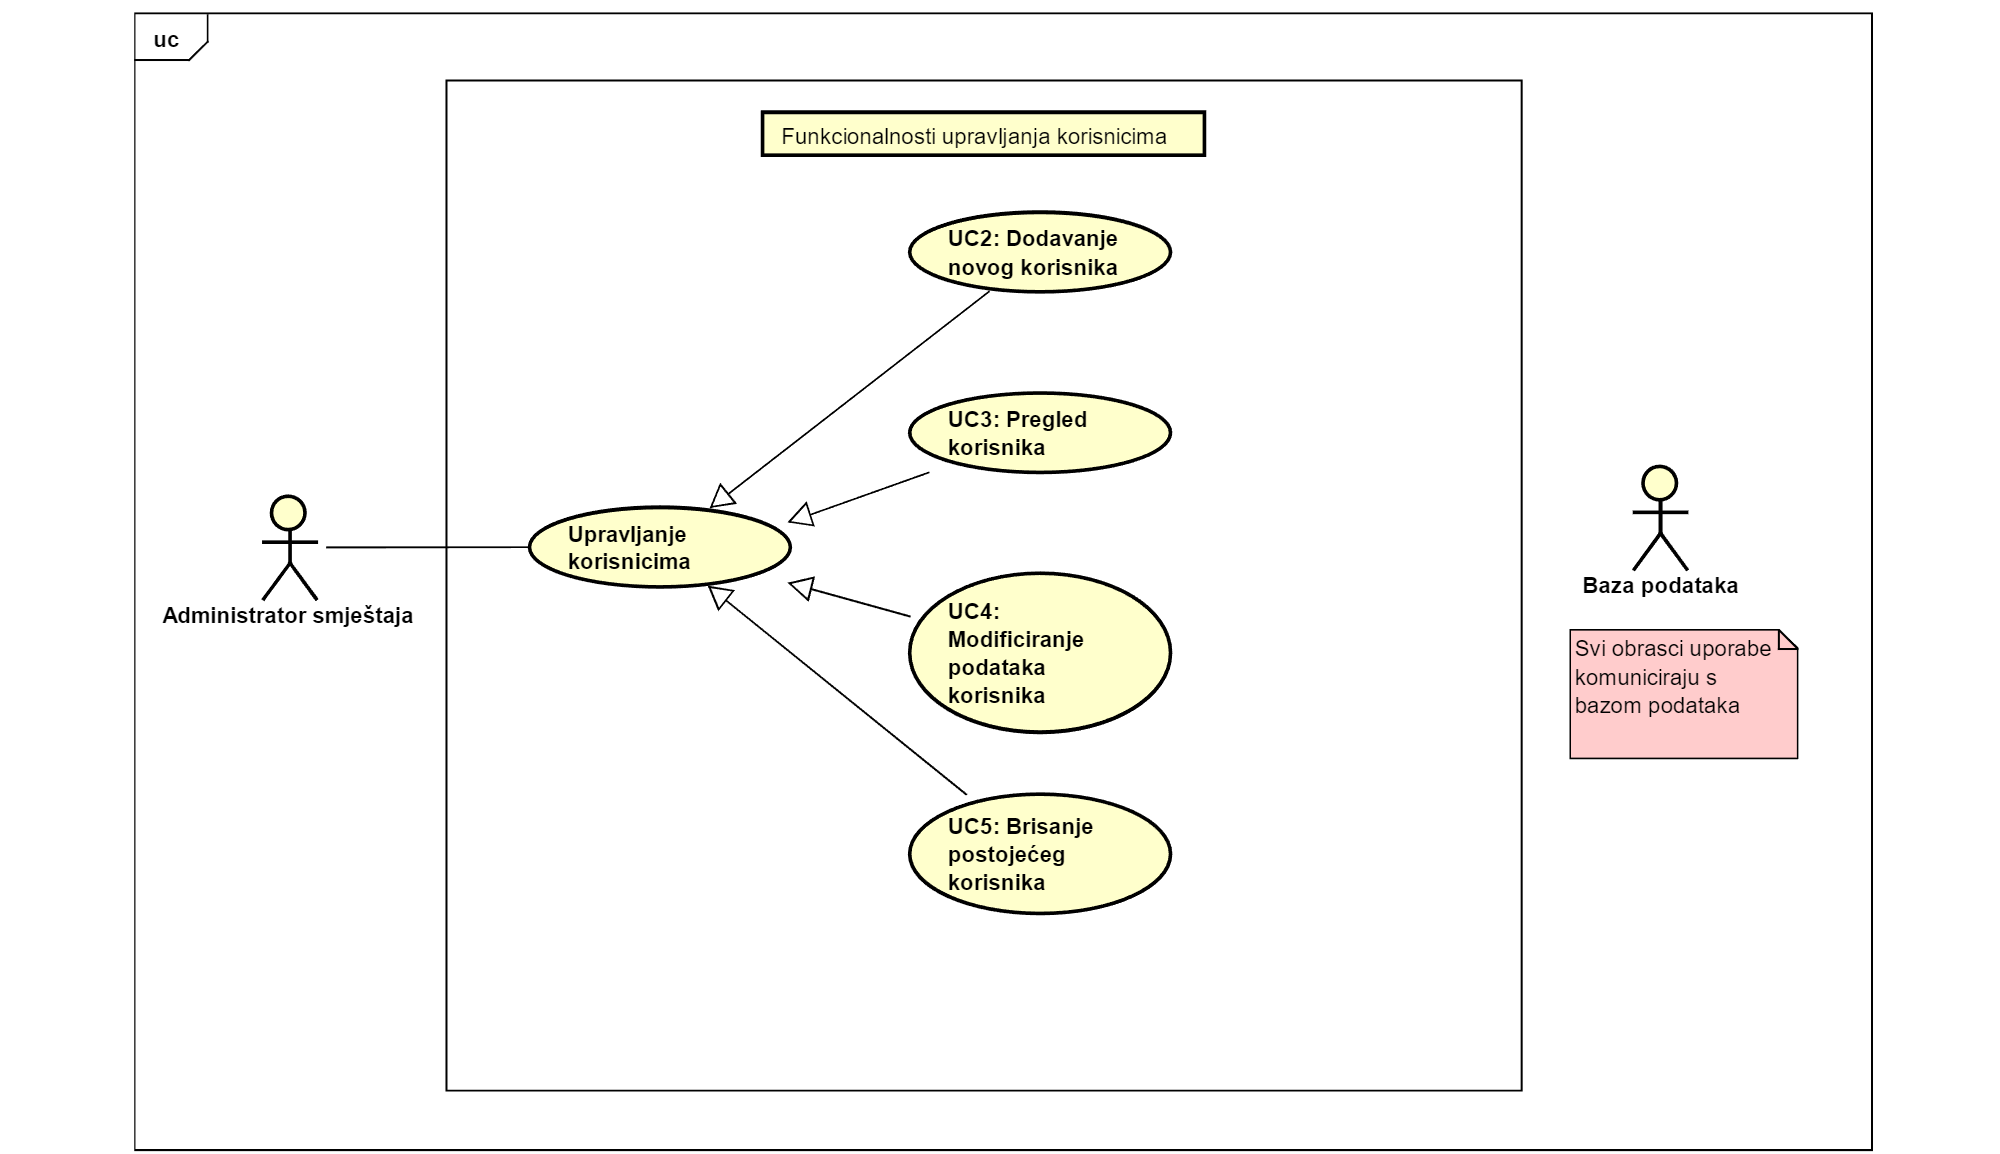
\includegraphics[width=\textwidth]{slike/DOU_FunkcionalnostiUpravljanjaKorisnicima.png} %veličina slike u odnosu na originalnu datoteku i pozicija slike
					\caption{Dijagram obrasca uporabe, funkcionalnosti upravljanja korisnicima}
					\label{fig:funkcionalnosti upravljanja korisnicima}
				\end{figure}
				\eject		
				
					\begin{figure}[H]
					\centering
					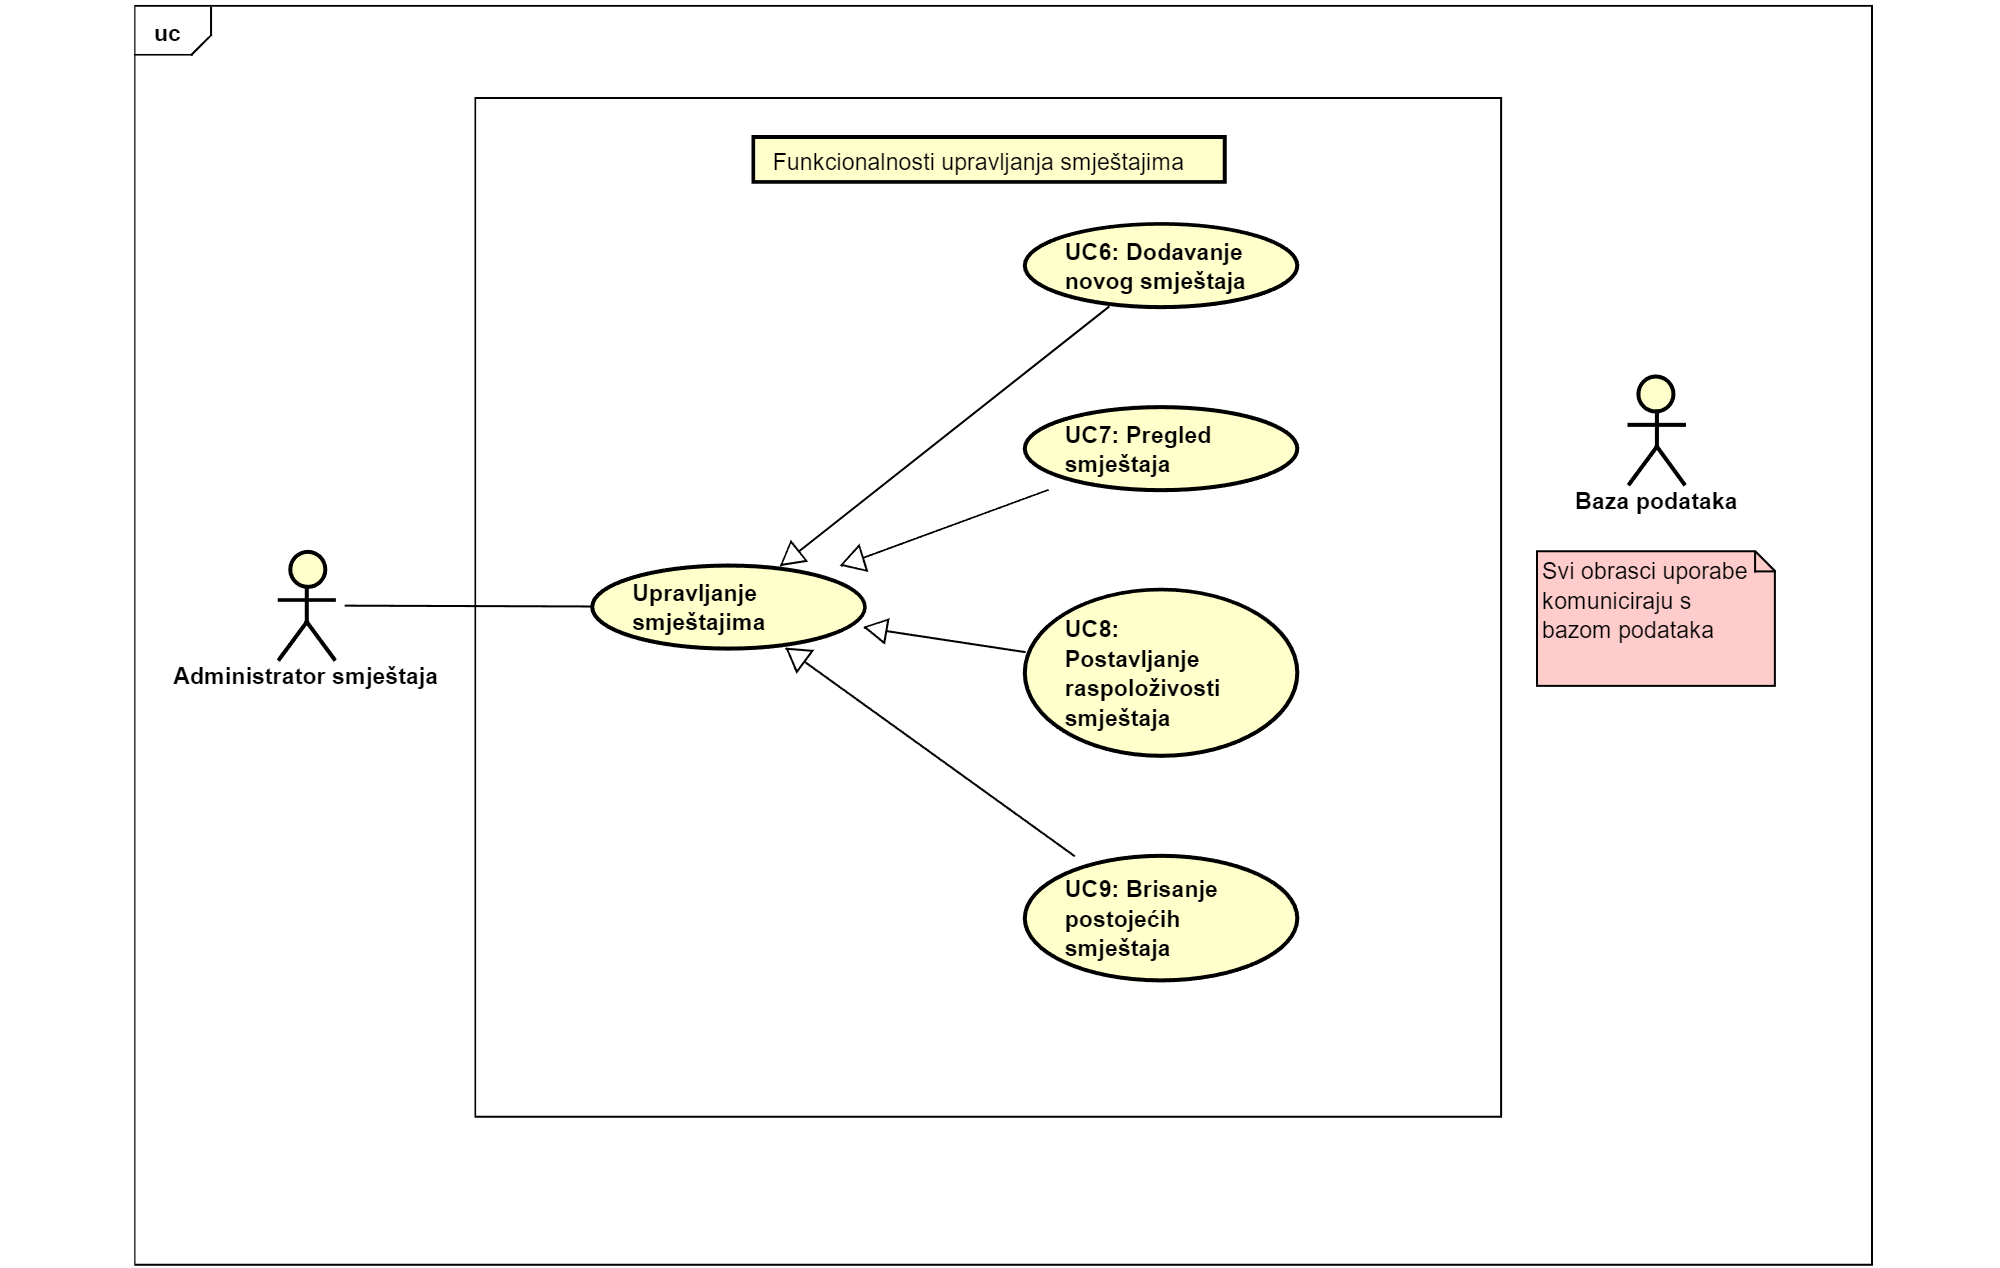
\includegraphics[width=\textwidth]{slike/DOU_FunkcionalnostiUpravljanjaSmjestajima.png} %veličina slike u odnosu na originalnu datoteku i pozicija slike
					\caption{Dijagram obrasca uporabe, funkcionalnosti upravljanja smjestajima}
					\label{fig:funkcionalnosti upravljanja smjestajima}
				\end{figure}
				\eject		
				
				\begin{figure}[H]
					\centering
					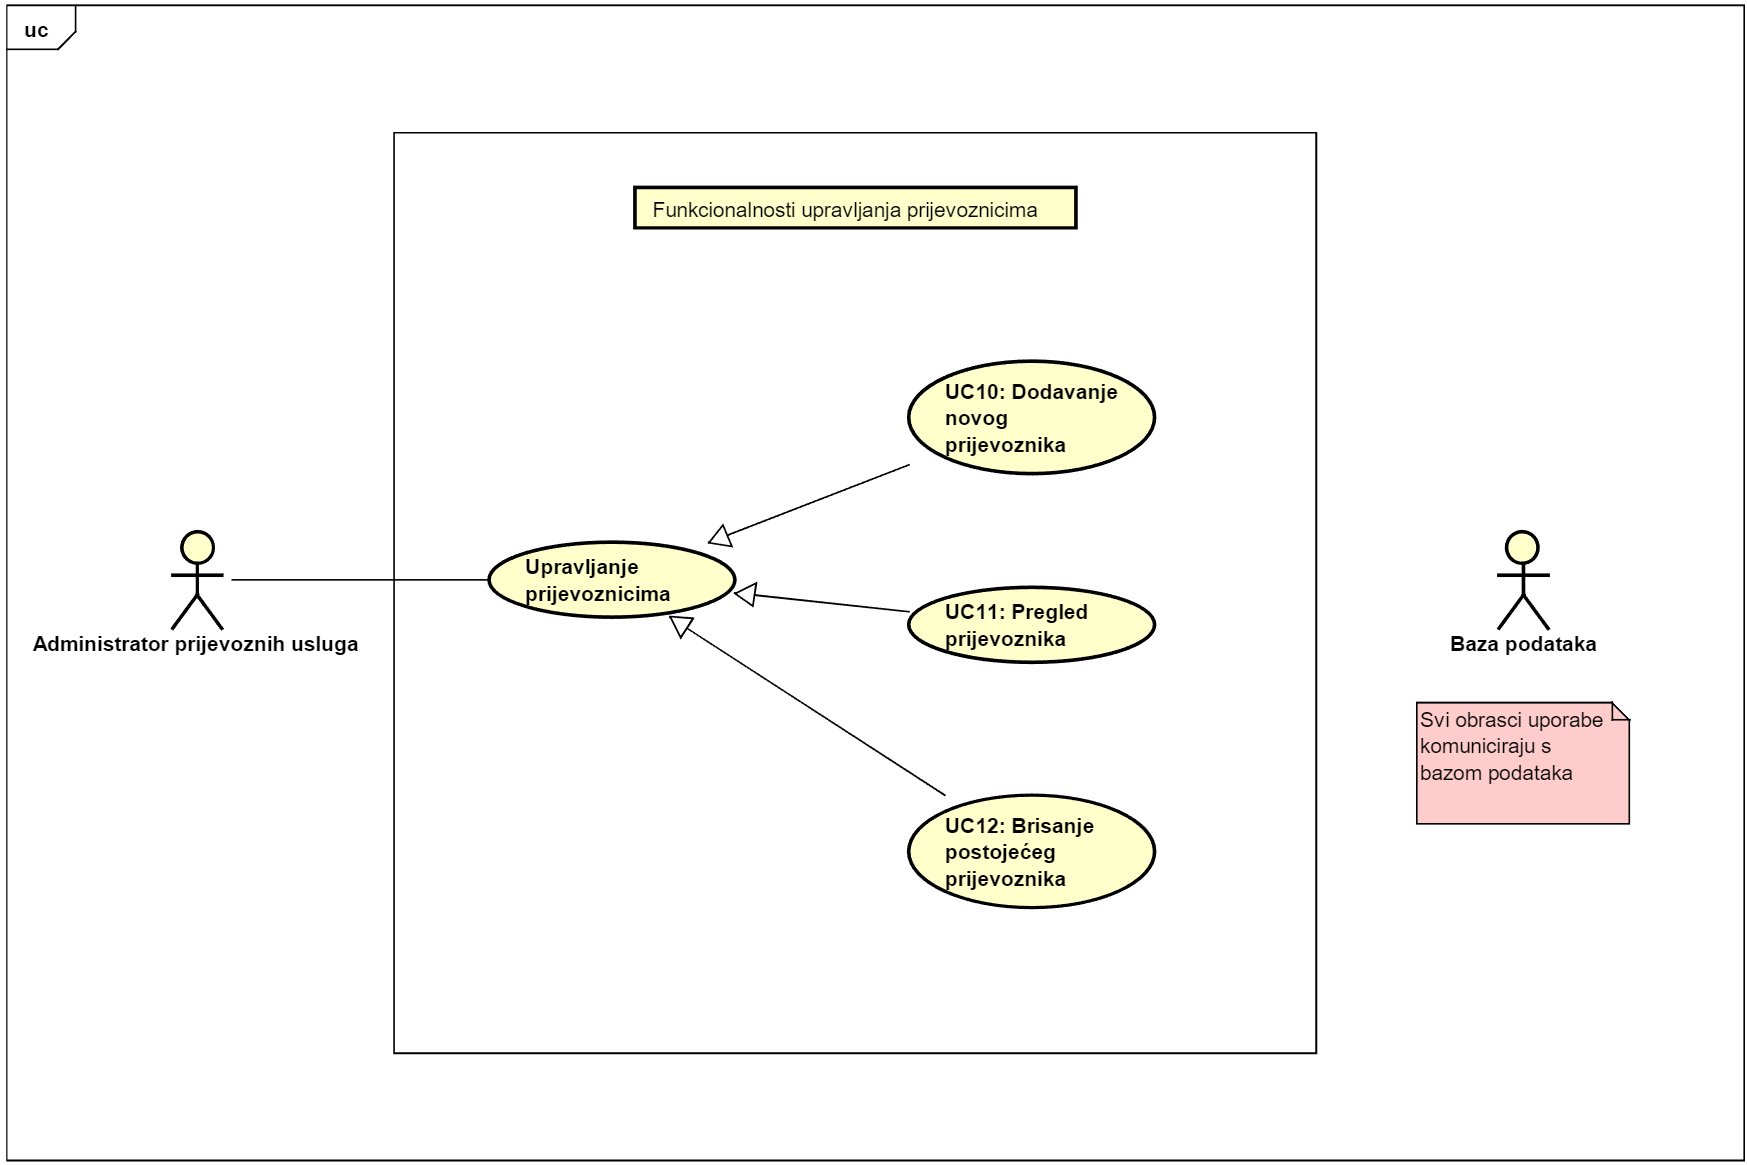
\includegraphics[width=\textwidth]{slike/DOU_FunkcionalnostiUpravljanjaPrijevoznicima.png} %veličina slike u odnosu na originalnu datoteku i pozicija slike
					\caption{Dijagram obrasca uporabe, funkcionalnosti upravljanja prijevoznicima}
					\label{fig:funkcionalnosti upravljanja prijevoznicima}
				\end{figure}
				\eject		
				
				\begin{figure}[H]
					\centering
					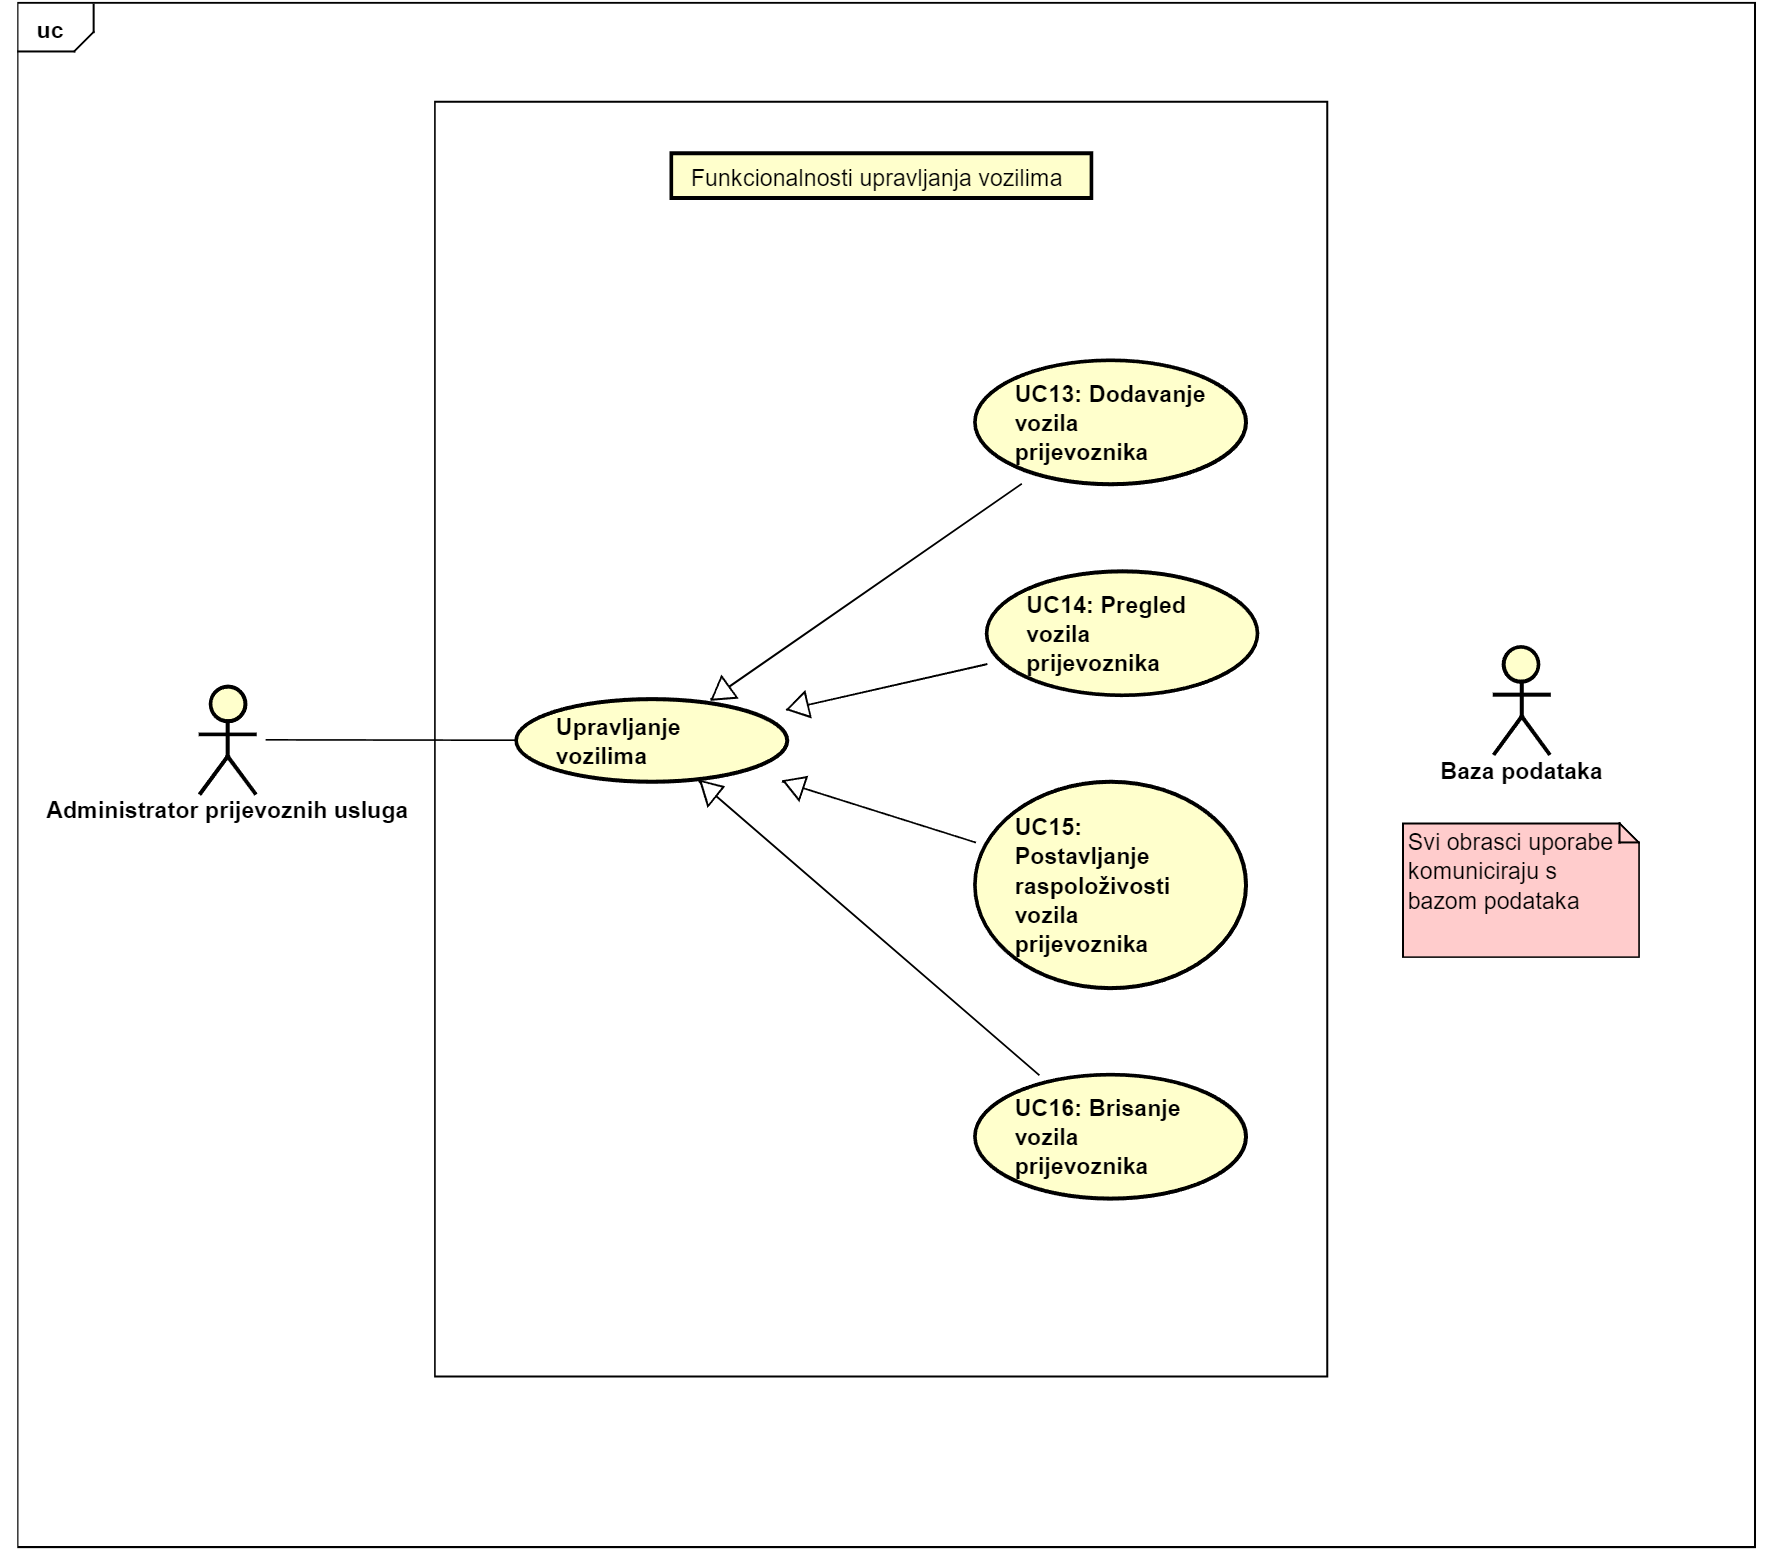
\includegraphics[width=\textwidth]{slike/DOU_FunckionalnostiUpravljanjaVozilima.png} %veličina slike u odnosu na originalnu datoteku i pozicija slike
					\caption{Dijagram obrasca uporabe, funkcionalnosti upravljanja vozilima}
					\label{fig:funkcionalnosti upravljanja vozilima}
				\end{figure}
				\eject		
				
				\begin{figure}[H]
					\centering
					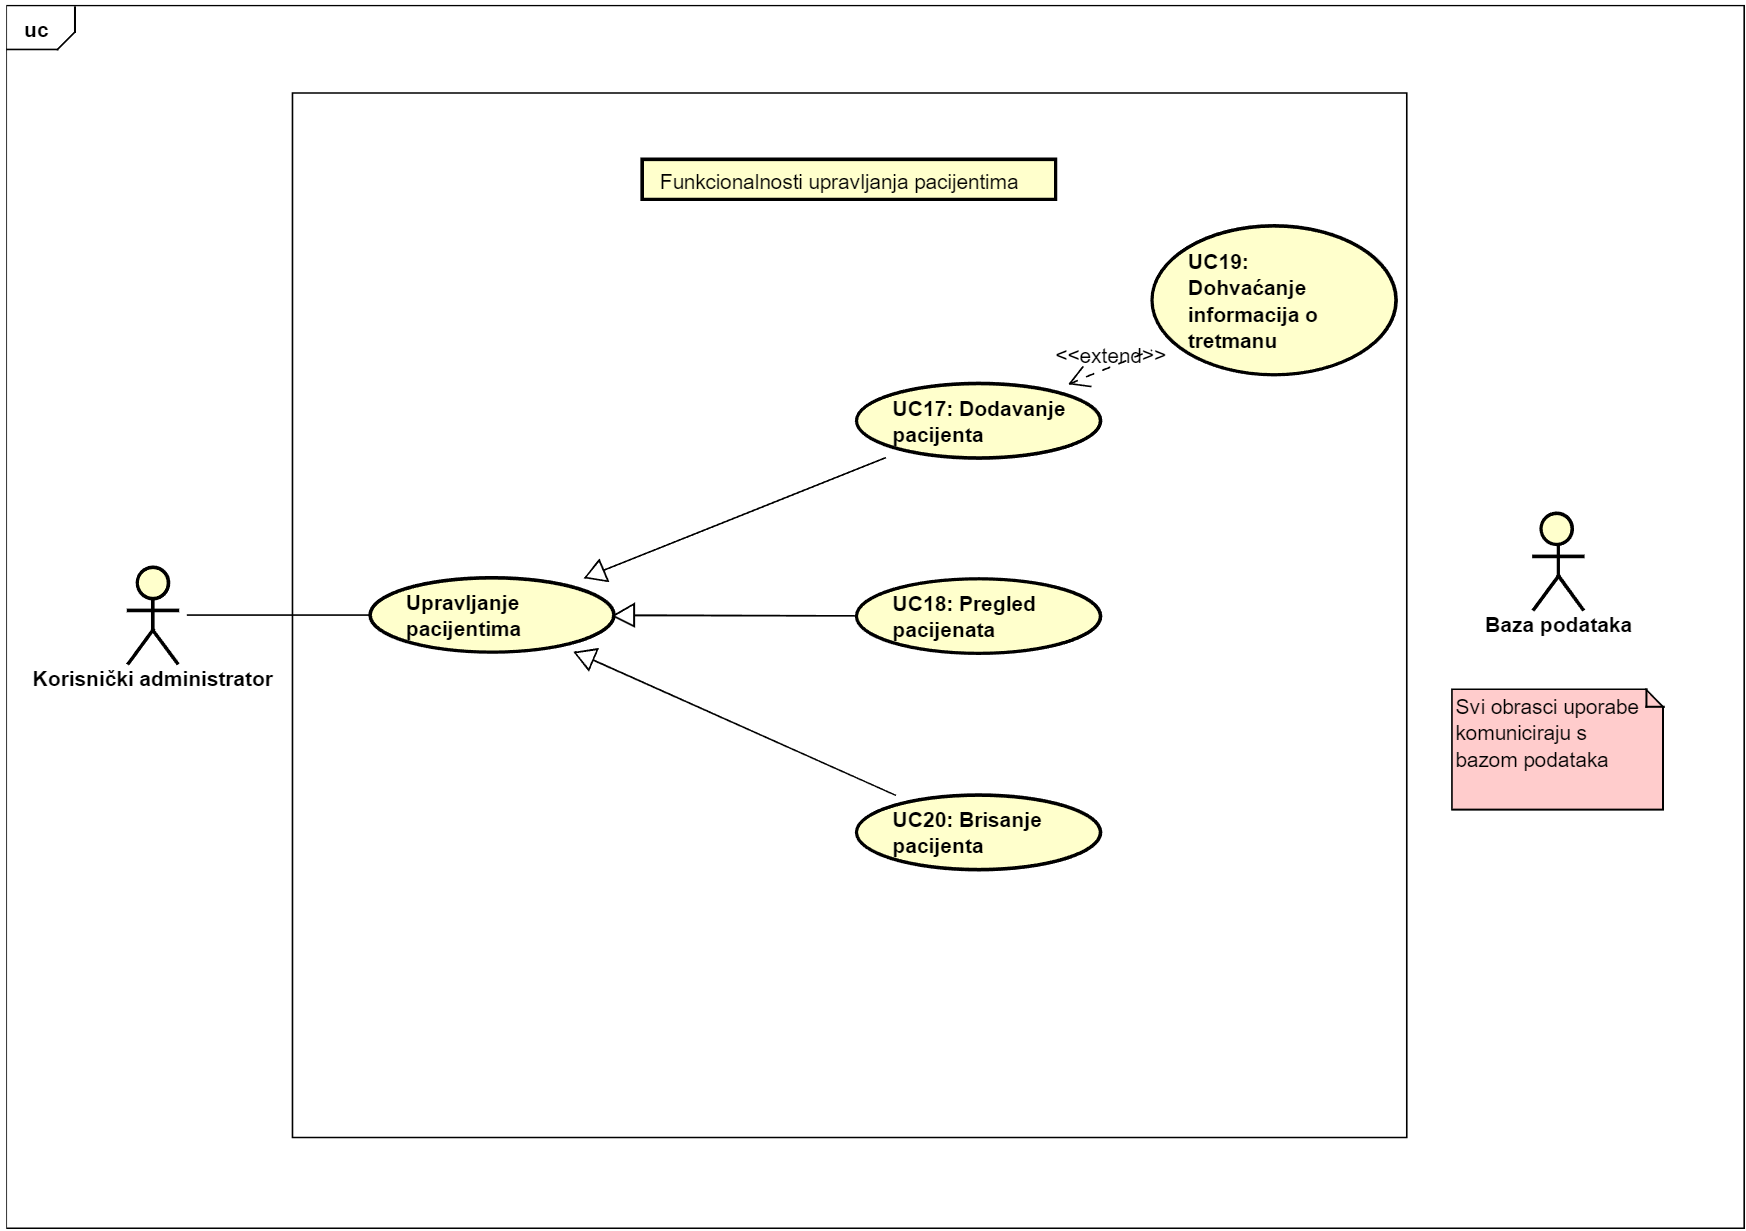
\includegraphics[width=\textwidth]{slike/DOU_FunckionalnostiUpravljanjaPacijentima.png} %veličina slike u odnosu na originalnu datoteku i pozicija slike
					\caption{Dijagram obrasca uporabe, funkcionalnosti upravljanja pacijentima}
					\label{fig:funkcionalnosti upravljanja pacijentima}
				\end{figure}
				\eject		
				
				\begin{figure}[H]
					\centering
					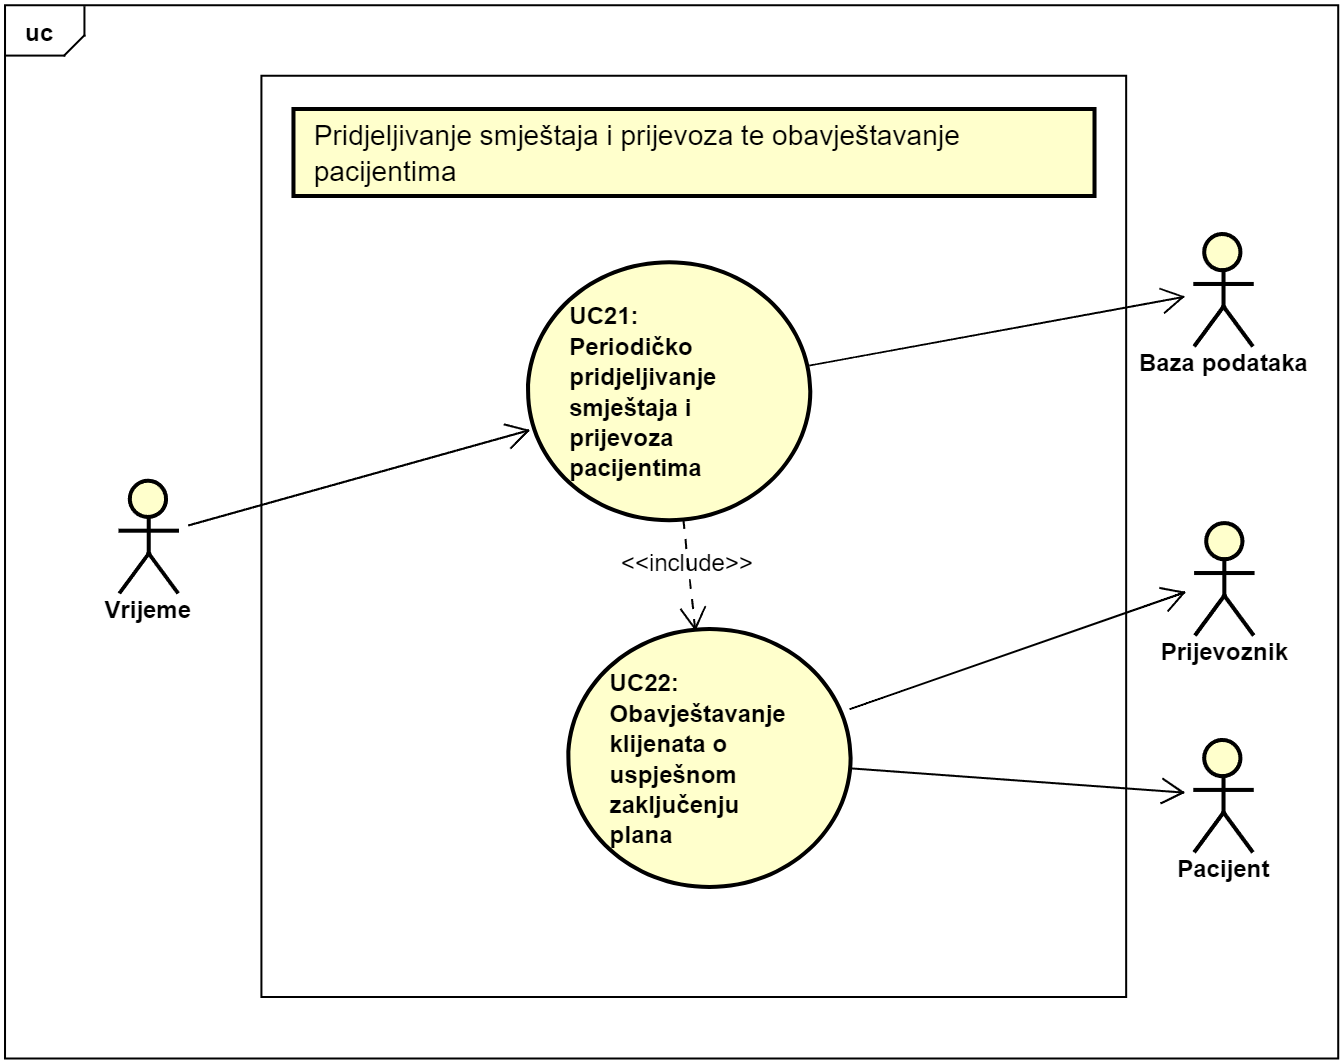
\includegraphics[width=\textwidth]{slike/DOU_UC21UC22.png} %veličina slike u odnosu na originalnu datoteku i pozicija slike
					\caption{Dijagram obrasca uporabe, pridjeljivanje i obavještavanje}
					\label{fig:pridjeljivanje i obavještavanje}
				\end{figure}
				\eject		
				
			\subsection{Sekvencijski dijagrami}
				
				\textbf{\textit{dio 1. revizije}}\\
				
				\textit{Nacrtati sekvencijske dijagrame koji modeliraju najvažnije dijelove sustava (max. 4 dijagrama). Ukoliko postoji nedoumica oko odabira, razjasniti s asistentom. Uz svaki dijagram napisati detaljni opis dijagrama.}
				\eject
	
		\section{Ostali zahtjevi}
		
			\begin{packed_item}
				\item Sustav treba omogućiti rad više korisnika u stvarnom vremenu
				\item Korisničko sučelje i sustav moraju podržavati hrvatsku abecedu (dijakritičke znakove) pri unosu i prikazu tekstualnog sadržaja
				\item Izvršavanje dijela programa u kojem se pristupa bazi podataka ne smije trajati duže od nekoliko sekundi
				\item Sustav treba biti implementiran kao web aplikacija koristeći objektno-orijentirane jezike
				\item Neispravno korištenje korisničkog sučelja ne smije narušiti funkcionalnost i rad sustava
				\item Aplikacija treba biti jednostavna za korištenje, korisnici se moraju znati koristiti sučeljem bez opširnih uputa
				\item Nadogradnja sustava ne smije narušavati postojeće funkcionalnosti sustava
				\item Aplikacija kao valutu koristi EUR
				\item Veza s bazom podataka mora biti kvalitetno zaštićena, brza i otporna na vanjske greške
				\item Pristup sustavu mora biti omogućen iz javne mreže pomoću HTTPS.
			\end{packed_item}
			
		 
			 \textit{Nefunkcionalni zahtjevi i zahtjevi domene primjene dopunjuju funkcionalne zahtjeve. Oni opisuju \textbf{kako se sustav treba ponašati} i koja \textbf{ograničenja} treba poštivati (performanse, korisničko iskustvo, pouzdanost, standardi kvalitete, sigurnost...). Primjeri takvih zahtjeva u Vašem projektu mogu biti: podržani jezici korisničkog sučelja, vrijeme odziva, najveći mogući podržani broj korisnika, podržane web/mobilne platforme, razina zaštite (protokoli komunikacije, kriptiranje...)... Svaki takav zahtjev potrebno je navesti u jednoj ili dvije rečenice.}
			 
			 
			 
	